\chapter{Introduction}
\label{cap:introduction}

In this chapter we introduce the motivation and general idea of the project
addressed in this document, define its scope in the form of goals and non-goals,
and also how it is going to be approached.

\section{Motivation}

This project started as an attempt to bring features of code verification, in
the light-weight manner of systems such as Dafny \citep{DafnyManual}, to the
Elixir programming language which, from the point of view of a programmer, may
be also considered as a light-weight version of Erlang.

The choice of Elixir is twofold. On the one hand because it seems interesting to
apply verification techniques to a dynamically typed language and, on the other
hand, because Elixir is a suitable language for developing \gls{dsl}s, since we
can extend it with metaprogramming via macro expressions that are expanded at
compile time.

At the highest level, our idea is to provide macros to annotate Elixir code with
ghost (i.e. verification-related annotations), and to specify functions in the
form of preconditions and postconditions within a module. These annotations
would be removed before compiling the code of the functions into bytecode and,
once all of them had been collected, a verification process would verify them
also at compile-time as illustrated by Figure \ref{fig:diag}.

\begin{figure}[h]
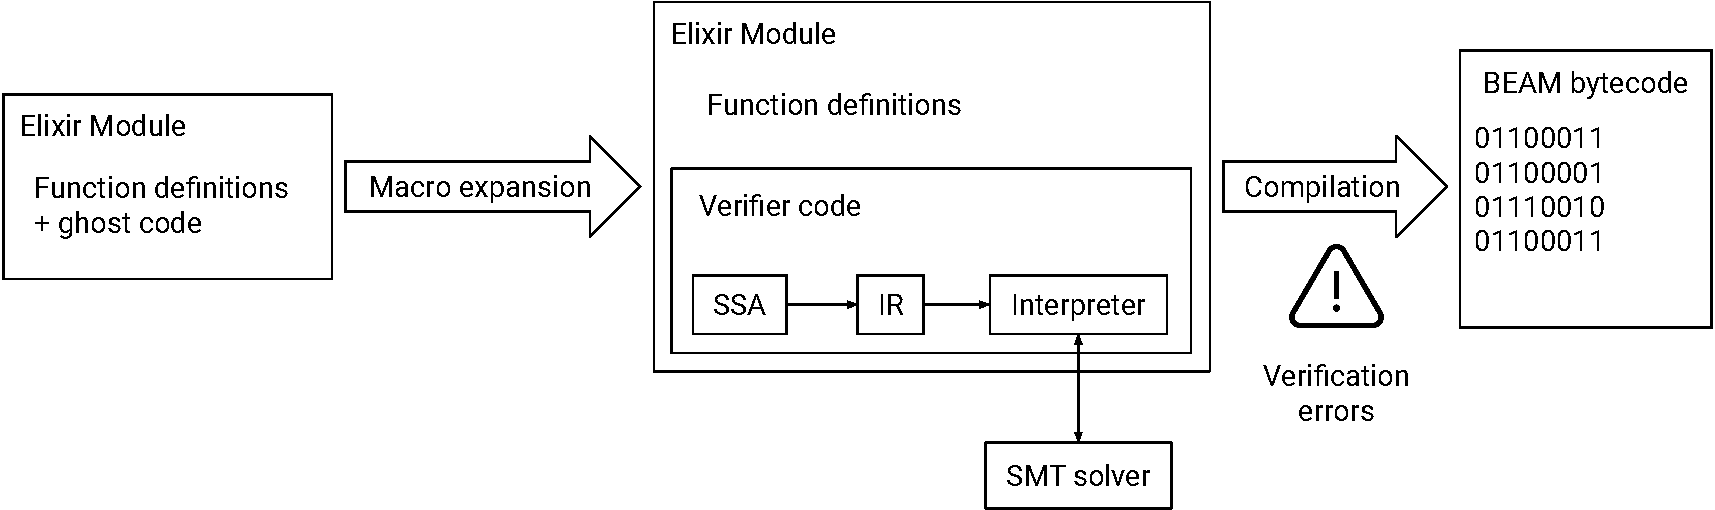
\includegraphics[width=\textwidth]{Images/Vectorial/Diagram}
\caption{Implementation diagram}
\label{fig:diag}
\end{figure}

A repository containing the code corresponding to this project is available
through the following URL:
\url{https://github.com/adrianen-ucm/verixir-project}.

\section{Goals}

The main goal of this project is to use the Elixir metaprogramming capabilities
through macros to implement a code verification system for the Elixir
programming language itself, without requiring us to modify its compiler or to
implement a parser.

Our system will rely on a verification \gls{ir} and the use of \acrshort{smt}
solvers for its verification.

\subsection{Sub-goals}

In order to achieve the main goal, we have proposed several possible sub-goals.
One of them is to integrate \acrshort{smt} solvers in Elixir with a \gls{dsl} of
macros, like in the following example that declares some sorts, functions and
constants, then adds to the solver state some formulas corresponding to the
theory of uninterpreted functions and linear arithmetic, and then checks the 
satisfiability of the solver state:

\begin{lstlisting}[language=elixir,numbers=none,frame=none]
declare_sort Term
declare_fun is_int: [term] :: Bool,
            int_val: [Term] :: Int

declare_const x: Term, 
              result: Term

assert :is_int.(:x)
assert :is_int.(:result)
assert :int_val.(:result) == :int_val.(:x) + :int_val.(:x)

check_sat
\end{lstlisting}

Another sub-goal is to develop a verification \gls{ir} to express Elixir terms
and their dynamically typed nature with simple constructs for verification, also
like in the following example:

\begin{lstlisting}[language=elixir,numbers=none,frame=none]
havoc x
havoc result

assume is_integer(x)
assume is_integer(result)
assume result === x + x
assert result === 2 * x 
\end{lstlisting}

We refer to our \gls{ir} by the name L1, as this project is divided in three
layers of abstraction.

Then, we must define a translation from this \gls{ir} into a simple language,
named L0, which is suitable to be verified by using our \acrshort{smt} solver
\gls{dsl}. This language offers control flow and failure signaling as in the
following example:

\begin{lstlisting}[language=elixir,numbers=none,frame=none]
declare x
declare result 

when_unsat is_boolean(is_integer(x)) do 
  add boolean_value(is_integer(x))
else 
  fail "Not a boolean"
end
\end{lstlisting}

Finally, we must also provide a mechanism to translate a subset of the Elixir
programming language together with ghost verification expressions, named L2,
into the verification \gls{ir}. We must also offer an \gls{api} for allowing its
usage when writing Elixir code like in the following example:

\begin{lstlisting}[language=elixir,numbers=none,frame=none]
@verifier requires is_integer(x)
@verifier ensures is_integer(dup(x)) and dup(x) === 2 * x
defv dup(x) do
  x + x
end
\end{lstlisting}

\subsection{Non-goals}

We have left some points as possible future work. The first one is that we are
going to deal only with sequential Elixir programs and not with concurrent ones.
Even for the sequential Elixir part we are going to support only a small subset 
to start with. Some non supported features are for example exceptions,
higher-order functions and the Elixir \verb|pin| operator.

Also, we are going to deal only with partial verification for the moment and not
with termination. Nevertheless, we will discuss some ideas regarding the latter
when introducing user-defined verification functions and how the system allows
to unfold their invocations. We also mention these topics in Chapter
\ref{cap:conclusions}, which shows the conclusions of this project and future
work.

\section{Work plan}

As a work plan, we will address the sub-goals as follows, preceded by a training
period for acquiring the required knowledge and practice with the Elixir
programming language.

Chapter \ref{cap:stateOfTheArt} shows the current research, tools and techniques
related to our project, and Chapter \ref{cap:preliminaries} introduces the
required tools and concepts, mainly Elixir and \acrshort{smt} solvers, both
chapters corresponding to the training period. Chapter
\ref{cap:smtSolverIntegration} presents our \acrshort{smt} solver integration
for Elixir and a formalization that will allow us to verify expressions of our
\gls{ir}, which is addressed in Chapter \ref{cap:intermediateRepresentation}.
Finally, Chapter \ref{cap:elixirCodeVerification} shows the verification system
and a preliminary overview of the resulting tool.
